
%(BEGIN_QUESTION)
% Copyright 2006, Tony R. Kuphaldt, released under the Creative Commons Attribution License (v 1.0)
% This means you may do almost anything with this work of mine, so long as you give me proper credit

Forklar hvordan gain-justeringen virker i denne pneumatiske proporsjonalregulatormekanismen:

$$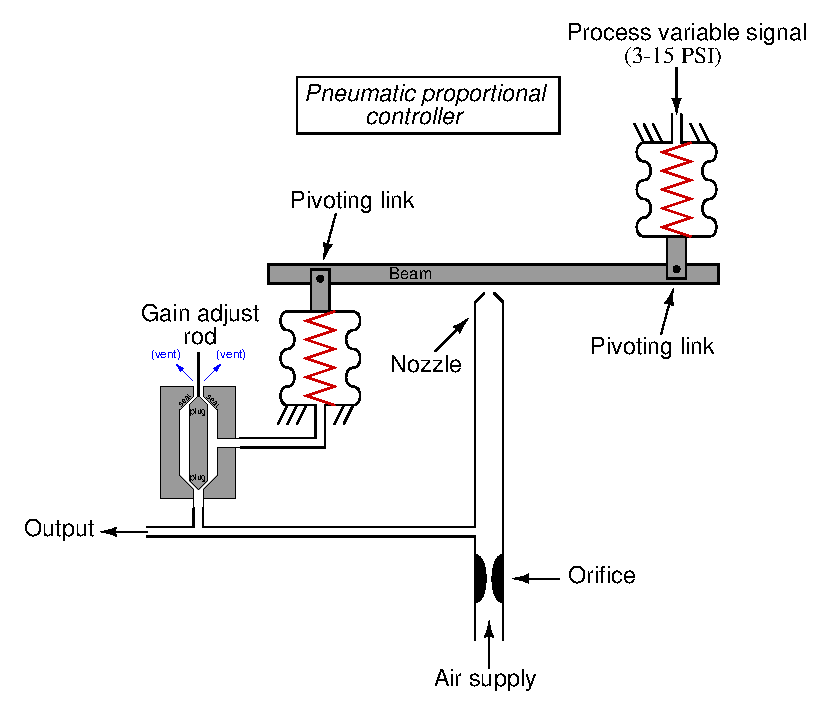
\includegraphics[width=15.5cm]{i01482x01.eps}$$

Ved å flytte ``gain adjust rod'' opp og ned kan regulatorens gain varieres. Angi hvilken bevegelsesretning som gir {\it høyere} gain.

\vskip 20pt \vbox{\hrule \hbox{\strut \vrule{} {\bf Forslag til sokratisk diskusjon} \vrule} \hrule}

\begin{itemize}
\item{} Angi minst én fordel denne metoden for gain-justering har sammenlignet med andre gain-justeringsmetoder du har sett i pneumatiske regulatormekanismer.
\item{} Anta at denne pneumatiske regulatormekanismen ble utvidet med et {\it forsterkende relé} for å forbedre ytelsen. Hvor nøyaktig i mekanismen ville det nye reléet blitt plassert?
\item{} Hvordan ville denne regulatormekanismen oppført seg hvis strupingen ble flyttet til en plassering mellom utgangsrøret og dysen, i stedet for mellom luftforsyningen og utgangsrøret der den skal være?
\item{} Skisser en elektronisk op-amp-krets med justerbar gain som virker analogt med denne pneumatiske regulatormekanismen.
\end{itemize}

\underbar{file i01482}
%(END_QUESTION)





%(BEGIN_ANSWER)

Tips: den pneumatiske {\it pilot}-mekanismen er analog med et elektrisk potensiometer koblet som spenningsdeler.

\vskip 10pt

For å se en elektrisk analogi av denne mekanismen, skisser en op-amp-krets med negativ tilbakekobling der den inverterende inngangen får en andel av utgangsspenningen via et potensiometer.

%(END_ANSWER)





%(BEGIN_NOTES)

Når stangen flyttes {\it nedover}, tilbakekobles minst utgangstrykk til belgen, og regulatorens gain øker. Dette ligner tilbakekoblingsnettet i en operasjonsforsterkerkrets, der en mindre tilbakekoblet andel av utgangssignalet tvinger utgangssignalet til å endre seg mer enn ellers (altså høyere total gain).

\vskip 10pt

Dette regulator-designet er løst basert på Fisher ``Multi-Trol'', med samme gain-justeringsmekanisme og samme bevegelsesbalanseoppsett.

\vskip 10pt

Ved å bruke variabel pneumatisk signaltilbakekobling for å styre gain i mekanismen blir det mulig med {\it fjernjustering av gain}.







\vfil \eject

\noindent
{\bf Oppsummeringsquiz:}

For å øke {\it gain} i denne regulatoren må man:

$$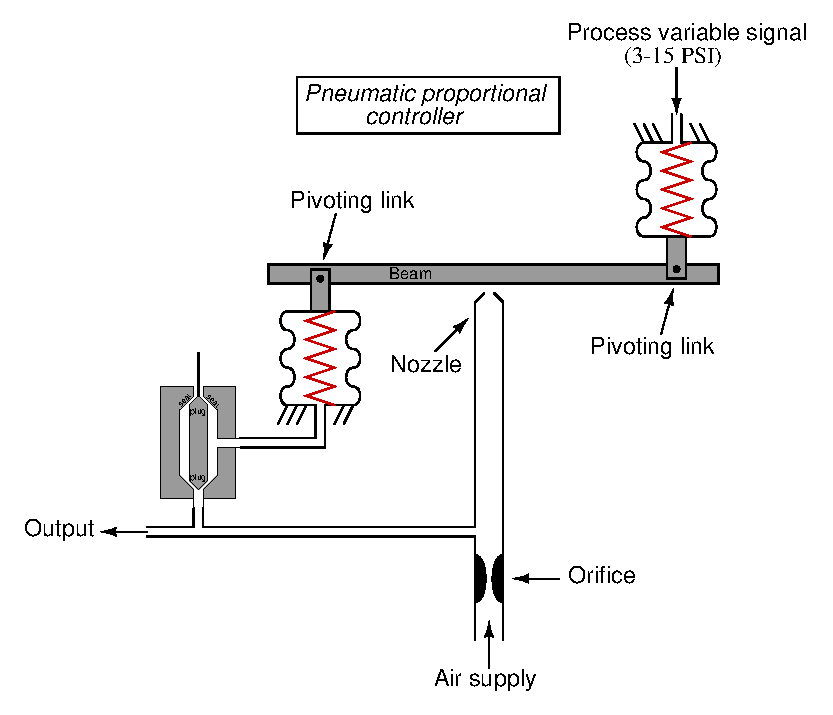
\includegraphics[width=15.5cm]{i01482x02.eps}$$

\begin{itemize}
\item{} Flytte dysen nærmere armen (klaffen)
\vskip 5pt 
\item{} Flytte pluggen i pilotventilen nedover
\vskip 5pt 
\item{} Øke trykket i trykkluftforsyningen
\vskip 5pt 
\item{} Senke trykket i trykkluftforsyningen
\vskip 5pt 
\item{} Flytte pluggen i pilotventilen oppover
\vskip 5pt 
\item{} Flytte dysen lenger bort fra armen (klaffen)
\end{itemize}


%INDEX% Control, proportional: pneumatic motion-balance controller

%(END_NOTES)

